\documentclass[10pt]{article}
\usepackage[right=2cm,left=2cm,top=2cm,bottom=3cm]{geometry}
\usepackage[utf8]{inputenc}
\usepackage[spanish]{babel}
\usepackage{amsmath}
\usepackage{color}
\usepackage{listings}
\usepackage{graphicx}
%\usepackage{multicol}

%COLORES CODIGO
\definecolor{gray97}{gray}{.97}
\definecolor{gray75}{gray}{.75}
\definecolor{gray45}{gray}{.45}
\definecolor{claregreen}{RGB}{4,180,95}
\definecolor{darkblue}{rgb}{0.0,0.0,0.6}


\lstset{ frame=Ltb,
     framerule=0pt,
     aboveskip=0.5cm,
     framextopmargin=3pt,
     framexbottommargin=3pt,
     framexleftmargin=0.4cm,
     framesep=0pt,
     rulesep=.4pt,
     backgroundcolor=\color{gray97},
     rulesepcolor=\color{black},
     %
     stringstyle=\ttfamily,
     showstringspaces = false,
     basicstyle=\small\ttfamily,
     commentstyle=\color{gray45},
     keywordstyle=\bfseries,
     %
     numbers=left,
     numbersep=15pt,
     numberstyle=\tiny,
     numberfirstline = false,
     breaklines=true,
   }

% minimizar fragmentado de listados
\lstnewenvironment{listing}[1][]
   {\lstset{#1}\pagebreak[0]}{\pagebreak[0]}

%LENGUAJE OZ
\lstdefinelanguage{OZ}
{
  morestring=[b]',
  morecomment=[s]{\%}{\%},
  stringstyle=\color{claregreen},
  keywordstyle=\color{blue}\bfseries,
  morekeywords={proc, end, \$},% list your attributes here
  emph={REQUIRED},
  emphstyle=\color{red}
}

%MODO CONSOLA
\lstdefinestyle{consola}
   {basicstyle=\scriptsize\bf\ttfamily,
    backgroundcolor=\color{gray75},
   }




%opening
\title{Simulación de Eventos Discretos.\\ \emph{Informe de Modelo e Implementación.} \\ \textbf{Simulación de Fallas de Máquinas.} }
\author{\textbf{María Andrea Cruz Blandón  0831816.} \\ \textbf{Edgar Andres Moncada 0832294.  }\\ \textbf{Luis Felipe Vargas Rojas 0836342. }}
\date{\today}







\begin{document}
\maketitle

\section{Análisis del Sistema y del Problema.}
\subsection{Descripción del Sistema}
El sistema esta compuesto de un conjunto de máquinas que funcionan en una fábrica, entre las cuales no existe conexión de manera que cada una trabaja independientemente de las otras; estas se mantienen encendidas 8 horas del día, es decir que el rendimiento total semanal se calcula con la fórmula $8*5*50$ donde 8 son las  horas del día, 5 son los días de la  semana, y 50 es el número de máquinas que están laborando.\\

Dentro de la fábrica se cuenta con un conjunto de máquinas adicionales que son enviadas a trabajar si alguna de las máquinas presenta una falla. También se cuenta con personal de mantenimiento que se encargan de reparar las máquinas que fallen; cada empleado puede reparar una máquina al tiempo, en caso de no tener a algún empleado disponible se debe poner en espera la máquina que falló, y en el momento de que un empleado la repare ésta se convierte en una máquina adicional.


\subsection{Descripción Gráfica del Sistema}
\begin{center}

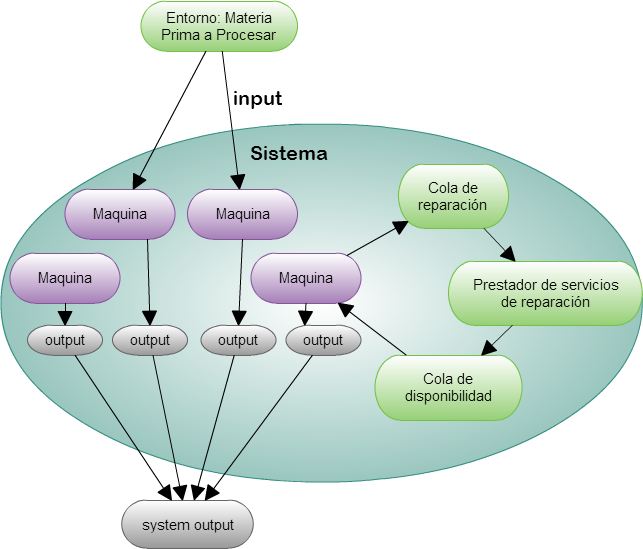
\includegraphics[scale=0.47]{Simulacion.png}

Figura1. \emph{Comportamiento del Sistema}
\end{center}

\subsection{Descripción del Problema}

La fábrica quiere mantener el stock de maquinaria principal en funcionamiento continuo por lo menos en un 96\% o 98\%. El problema que se tiene es que las máquinas son componentes que pueden presentar fallas, y estas afectan de manera general a la producción de la fábrica.\\

Para solucionar este problema la fábrica ha dispuesto de máquinas adicionales dispuestas a suplantar(REEMPLAZAR) las máquinas que se dañen durante el proceso, que tienen a fallar luego de $160\pm30$ horas. También se cuenta con un equipo de mantenimiento que puede reparar, las máquinas que se dañen, en aproximadamente $8\pm3$ horas. Sin embargo no siempre son suficientes las máquinas auxiliares y la cantidad de personal para atender las máquinas que fallan y mantener la utilidad requerida de funcionamiento de las 50 maquinas. Por esta razón la fábrica quiere determinar cuántas máquinas adicionales y cuánto personal es el necesario para cumplir la meta.

\section{Modelo de Simulación.}

\subsection{Simulación en general}

Puntos claves:
\begin{itemize}
\item Cada máquina de la fábrica tiene la probabilidad de fallar en un periodo de $160\pm30$ horas con una distribución uniforme.
\item La cantidad de reparadores puede variar según los escenarios planteados.
\item La cantidad de máquinas adicionales puede variar según los escenarios planteados.
\item Es adecuado realizar un tiempo de calentamiento ya que existe formación de colas.
\item Una máquina que se esté reparando o esté esperando para ser reparada no puede generar un evento de fallo, pues no está en funcionamiento. 
\end{itemize}

Al iniciar la simulación se genera un evento de fallo por cada una de las máquinas de la fábrica. Estos eventos se generan con un  espacio de $20$ horas. Esto es con el fin de evitar la situación: \emph{Todas las máquinas fallan a la vez}. Una vez se tiene este conjunto de eventos, se realiza el período del calentamiento, este consiste en realizar la simulación hasta 


\subsection{Eventos.}

\begin{itemize}
\item Fallo de una máquina.
\item Reparación de una máquina.
\end{itemize}

Diagramas de flujo de los eventos:
\begin{center}

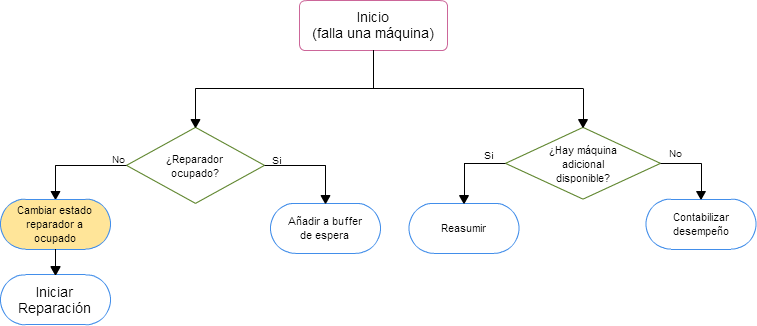
\includegraphics[scale=0.47]{fallaMaquina.png}

Figura2. \emph{Evento: Se presenta una falla en una de las máquina.}
\end{center}
\begin{center}

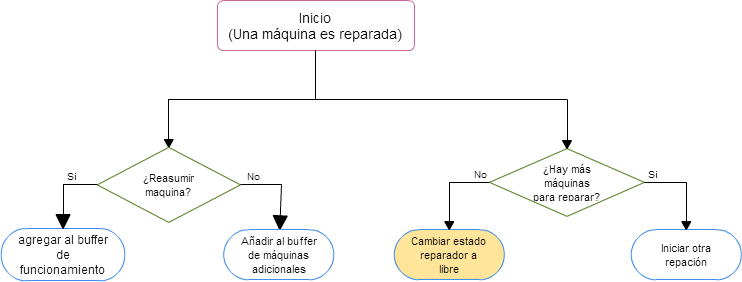
\includegraphics[scale=0.47]{reparar.png}

Figura3. \emph{Evento: Se realiza la reparación de una de las máquinas dañadas.}
\end{center}



\subsection{Reloj de La Simulación}

La unidad de tiempo que se va a emplear es la hora. El reloj va a avanzar de acuerdo al modelo de simulación LEF, donde se almacenan los tiempos de los eventos futuros y se ordenan cronológicamente, así el cambio de estado del reloj  se va a dar por el tiempo del evento más próximo en cada iteración.\\

La simulación termina cuando:
\begin{enumerate}
\item El reloj del sistema a llegado a un valor indicado.
\item No hay mas eventos futuros en la lista de eventos.
\end{enumerate}

\subsection{Comportamiento de los Datos.}

\begin{itemize}
\item \textbf{Fallo de una maquina:}\\
Se verifica si existe un reparador disponible, si lo hay éste pasa a estar ocupado reparando la máquina que falló; sino la máquina pasa a una cola de espera para ser reparada.
Además se debe precisar: si hay una máquina adicional disponible esta debe reemplazar la máquina que falló, sino la hay el rendimiento disminuye en una unidad (una máquina menos trabajando).


\item \textbf{Reparación de una maquina:}\\
Si al terminar una reparación hay máquinas en espera de reparación el técnico inicia una nueva reparación, por lo que la cola de espera disminuye en una unidad. También se debe verificar si
la máquina reparada entra en la lista de máquinas adicionales o pasa a reemplazar una máquina que halla fallado.

Si al terminar una reparación no hay más máquinas que reparar se desocupa el técnico de reparación.

\end{itemize}



\section{Diseño y Analisis de Escenarios.}


\section{Implementación del Modelo.}




\section{Conclusiones.}



\end{document}

